\chapter{Analiza numeryczna i~symulacja systemów}
\PartialToc
%\startcontents[chapters]
%\printcontents[chapters]{}{1}{\section*{\contentsname}}
\section{EKK\_1}
\textbf{Wskaż prawidłowo sformułowane warunki w zagadnieniach początkowych Cauchy'ego (IVP) dla równania różniczkowego $y'(t) = f(t, y(t)), f: \Omega \subset \Re \times \Re^{n} \shortrightarrow \Re^{n}, t \in [a, b]$.}

\vspace{0.4cm}
\noindent  Warunki początkowe do para $(t_0, y_0) \in \Omega$. Może to być para wektorów, jeśli mamy do czynienia z równaniem wielu zmiennych: $y=[y_1, y_2, ..., y_n]$. Dla wszystkich wartości $y_i$ potrzebujemy wartości początkowych (tj. w punkcie $a$). Wartości na krańcach przedziału są wykorzystywane w zagadnieniach brzegowych (BVP). Odpowiedź przykładowa miesza problem dwóch zmiennych z problemem BVP. 
Przykłady odpowiedzi:
$$n=2, y_{10}=y_1(a), y_{20}=y_2(a)$$
$$n=1, y_0=y(a)$$
%\begin{center}
%
\includegraphics[width=6cm]{buka}
%\captionof{figure}{Buka}
%\end{center}


\section{EKK\_1, EKK\_18}
\textbf{Wskaż diagramy SIMULINK'a, które reprezentują równanie różniczkowe $$y''-2y'+7y=3sin(5t)-1$$}

\vspace{0.4cm}
\noindent Rysunek tłumaczy wszystko. Centralną częścią jest to wielkie kółko. Ono zamyka pętle i wymusza prawdziwość równości. Analogiczny obrazek można zrobić z blokami Derivative (różniczkującymi), ale dla równania $y=\frac{3sin(5t)-1+2y'-y''}{7}$ współczynniki są brzydsze (mało ''naturalne'').
\begin{center}
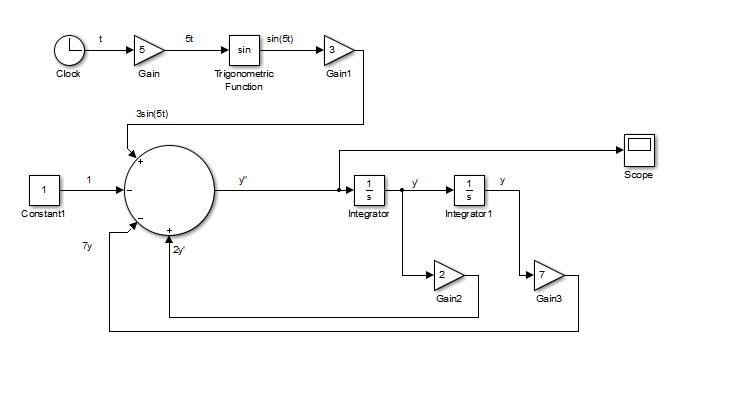
\includegraphics[width=15cm]{08/simulink}
\captionof{figure}{Simulink}
\end{center}
\newpage
\section{EKK\_1}
\textbf{Które zdania odnoszące się do metod rozwiązywania zagadnień początkowych dla równań różniczkowych są prawdziwe?}

\vspace{0.4cm}
\noindent
Metoda trapezowa jest jednokrokowa.\\
Metoda Heuna jest jednokrokowa, dwuetapowa - blok w SIMULINK'u $heun$.\\
Metoda Adamsa-Bashforta jest wielokrokowa, jednoetapowa, jawna.\\
Metoda BDF (Gear'a, wstecznego różniczkowania) jest wielokrokowa, jednoetapowa, jawna - komenda $ode15s$.\\
Metoda Adamsa-Bashforta-Moultona jest wielokrokowa, dwuetapowa - komenda $ode113$.\\
Metoda Milne-Simpsona jest rzadko stosowana ze względu na swój brak stabilności.\\
Obecnie nazwą metody Rungego-Kutty określa się rodzinę jawnych i niejawnych metod wielokrokowych, jak również pewne ich modyfikacje. \\
Tu chodzi o tak zwane metody wielokrokowe (potrzebujemy pamiętać kilka poprzednich stanów, a nie tylko jeden ostatni - dla 6-krokowej metody wzór może wyglądać na przykład tak: $y_{n+1}=y_n+\frac{h}{1440}(4277f_n-7923f_{n-1}+2616f_{n-2}-7298f_{n-3}+2877f_{n-4}-475f_{n-5})+O(h^7)$).
Metoda jednokrokowa korzysta tylko z $y_n$.\\
Metody dwuetapowa korzysta z dwu takich wzorów jak powyższy. Każdy wzór to jeden etap.
Metody niejawne mają po prawej stronie $f_{n+1}$, do którego policzenia potrzebujemy $y_{n+1}$. A $y_{n+1}$ właśnie chcemy policzyć z tego wzoru. No i stąd ta niejawność wzoru.

\section{EKK\_1}
\textbf{Numeryczne rozwiązywanie zagadnienia początkowego. Która metoda jest metodą samostartującą:}

\vspace{0.4cm}
\noindent Eulera, Rungego-Kutty.
Adamsa-Bashforta-Moultona i Geara nie.

\section{EKK\_1}
\textbf{W przypadku metody Eulera zastosowanej do rozwiązywania zagadnienia początkowego dla $y'(t)=f(t,y(t)), y_0=y(0)$ (przy założeniu braku błędu numerycznego wszystkich operacji arytmetycznych)}

\vspace{0.4cm}
\noindent Równanie różniczkowe $\frac{dy}{dx}=f(x,y(x))$ jest liniowe, jeśli $f(x,y(x))=p(x)y+q(x)=Ay+B.$\\
Dla metody Eulera korzystamy z tego, że:$$\frac{dy}{dx}=f(x,y(x)) \Leftrightarrow \frac{y_1-y_0}{h}=f(x,y) \Leftrightarrow y_1-y_0=hf(x,y).$$ To prowadzi do równości $y_{n+1}=y_n+hf(x,y)$.\\
Jak widać przypomina to rozwinięcie Taylora: $y(x_0+h)=y(x_0)+\frac{h}{1!}y'(x_0)+\frac{h^2}{2!}y''(x_0)+\frac{h^3}{3!}y'''(\xi)$, gdzie $\xi \in (x_0, x_0+h)$. Skoro jednak $f(x,y)$ jest funkcją liniową, zatem $y''(x_0)=f'(x,y)\neq0$ w ogólności (np. $f(x,y)=2x$ daje $f'(x,y)=2$). Błąd lokalny pierwszego kroku metody Eulera jest różny od zera, nawet jeśli równanie różniczkowe pierwszego rzędu jest liniowe.\\
Prawdą jest natomiast, że dla metody Eulera błąd lokalny jest proporcjonalny do kwadratu kroku, a błąd globalny - liniowy.

\newpage
\section{EKK\_1}
\textbf{Numeryczne rozwiązywanie zagadnienia początkowego. W metodach typu predyktor-korektor (PECE):}

\vspace{0.4cm}
\noindent Metody PECE to na przykład: Heuna, Adamsa-Bashforta-Moultona, Milne-Simpsona. Predykcja jest częścią jawną, korekcja niejawną. To są dwa etapy. Dlatego te metody są dwuetapowe.\\
Odpowiedź przykładowa, jakoby stosowało się metodę jawną lub niejawną jest nieprawidłowa. Stosuje się zawsze obie metody.

\section{EKK\_1}
\textbf{Które zdania, odnoszące się do metod Rungego-Kutty (RK) rozwiązywania zagadnienia początkowego dla równań różniczkowych, są prawdziwe}

\vspace{0.4cm}
\noindent Odpowiedź przykładowa jest nieprawdziwa. Wersja jawna 4-etapowej metody RK jest różny od wersji niejawnej choćby przez sam fakt istnienia po prawej stronie $f_{n+1}$ (patrz. 8.3.). Istnieją wersje 1-etapowe (to po prostu metoda Eulera), 2-etapowe (Heuna, punktu pośredniego), 4-etapowa jest najczęściej występująca (tę wersję ma się na myśli, gdy mówi się o metodzie RK). 

\section{EKK\_1}
\textbf{Jawne metody Rungego-Kutty (RK). Niech $n_e$ oznacza liczbę etapów metody, a $r$ - maksymalny osiągalny rząd metody.}

\vspace{0.4cm}
\noindent $r<=n_e$.

\section{EKK\_1}
\textbf{Algorytmy optymalizacji statycznej.}

\vspace{0.4cm} Optymalizacja statyczna - szukamy ekstremum funkcji.
Optymalizacja dynamiczna - szukamy ekstremum funkcjonału.\\
Metoda Neldera-Meada jest metodą bezgradientową, bo nie korzysta z pochodnych. Nadaje się więc także do funkcji nieróżniczkowalnych.
Numeryczne metody optymalizacji (deterministyczne): 
\begin{enumerate}
 \item bez ograniczeń:
 \begin{enumerate}
  \item bezgradientowe:
  \begin{itemize}
   \item simpleks Neldera-Meada,
   \item spadku względem współrzędnych (Gaussa-Seidla),
   \item Powella, Rosenbrocka, Hooke'a-Jeevesa;
  \end{itemize}
  \item gradientowe pierwszego rzędu:
  \begin{itemize}
   \item najszybszego spadku,
   \item gradientu sprzężonego;
  \end{itemize}
  \item gradientowe drugiego rzędu i ''superliniowe'':
  \begin{itemize}
   \item Newtona, BFGS,
   \item ''Trust region'';
  \end{itemize}
 \end{enumerate}
 \item z ograniczeniami:
 \begin{itemize}
  \item eliminacji zmiennych,
  \item Lagrange'a,
  \item z funkcją kary,
  \item SQP.
 \end{itemize}
\end{enumerate}

\section{EKK\_1, EKK\_U19}
\textbf{Dyskretna aproksymacja średniokwadratowa. Dla $n+1$ wartości zmiennej niezależnej $x_i, i=1,2,3,...,n, x_i<x_{i+1}$ wykonano pomiary i otrzymano $n+1$ wartości $y_i$. Zależność wielkości mierzonej od $x$ aproksymowano wielomianem $W_m(x)=\Sigma^m_{i=0}a_{i,m}x^i$ z błędem aproksymacji $E_m$. Proszę zaznaczyć prawdziwe implikacje:}

\vspace{0.4cm}
\noindent Aproksymacja oznacza przybliżanie funkcji $y=f(x)$ za pomocą "prostszej" funkcji $y=F(x)$. W zależności od sposobu obliczania błędu aproksymacji, dzielimy je na:
\begin{itemize}
\item jednostajne - błąd liczymy normą Czebyszewa: $ \textpipe\textpipe f-F\textpipe\textpipe =sup_{a<=x<=b}\textpipe\textpipe f(x)-F(x) \textpipe\textpipe ; $
\itemśredniokwadratowe - błąd liczymy: $ \textpipe\textpipe f-F\textpipe\textpipe = \int^{b}_{a}w(x)[f(x)-F(x)]^{2} dx .$
\end{itemize}
Skoro zebrano pomiary w $n+1$ punktach, a aproksymujemy wielomianem $m$-stopnia, to niekoniecznie otrzymamy błąd $E_m>0$. Możliwe jest, że punkty pomiarowe akurat tworzą wielomian $m$-stopnia (zupełnie jak trzy punkty na jednej prostej tworzą wielomian pierwszego stopnia, a nie drugiego). Jednakże implikacja zachodzi w drugą stronę:
$$E_m>0 \Rightarrow n>m.$$

\section{EKK\_1, EKK\_U19}
\textbf{Dla $n+1$ wartości zmiennej niezależnej $x_i, i=1,2,3,...,n,   x_i<x_{i+1}$ wykonano pomiary i otrzymano $n+1$ wartości $y_i$. Zależność wielkości mierzonej od $x$ aproksymowano wielomianem $W_m(x)=\Sigma^m_{i=0}a_{i,m}x^i$. Rozważamy 3 sposoby obliczania błędu aproksymacji $E_m$: 
\begin{enumerate}
\item $E_m=min_{a_0,\ldots,a_m}\Sigma^n_{i=0}\textpipe y_i - W_m(x_i) \textpipe$,
\item $E_m=min_{a_0,\ldots,a_m}\Sigma^n_{i=0}(y_i - W_m(x_i))^2$,
\item $E_m=min_{a_0,\ldots,a_m}max_{i=0,\ldots,n}\textpipe y_i - W_m(x_i) \textpipe$.
\end{enumerate}
Obliczenie współczynników $a_i$ można sprowadzić do zagadnienia liniowego:
}

\vspace{0.4cm}
\noindent Po wpisaniu w wyszukiwarkę Google hasła: ''Zagadnienie liniowe'' otrzymujemy wyniki, które wskazują jednoznacznie na synonimiczność z określeniem: "Programowanie liniowe"(za Wikipedią: ''Programowanie liniowe – klasa problemów programowania matematycznego, w której wszystkie warunki ograniczające oraz funkcja celu mają postać liniową.'').\\
Teraz pokrótce o aproksymacji. Opisano ją w sekcji wyżej, więc wystarczy nadmienić, że szukamy takich współczynników $a_i$, dla których błąd $E_m$ będzie możliwie najmniejszy. \\ 
Okazuje się, że nawet dla aproksymacji średniokwadratowej (opis sekcja wyżej) można sprowadzić problem do programowania liniowego (ciekawych odsyłam do \url{http://kik.weii.tu.koszalin.pl/aproksymacja/aproks_tryg/page_dyp/aprwielpaj.html}). Odpowiedzi 1. i 2. są więc prawidłowe. W przypadku ostatnim można zauważyć, że bierzemy obecny maksymalny błąd $a_i$ i staramy się go zmiejszyć. Norma nie pomaga jednak zwięźle opisać algorytmu (kiedy założyć stop algorytmu, skoro musimy sprawdzić wszystkie możliwe kombinacje, by zminimalizować maksymalne odchylenie?). Wynikałoby z tego, że odpowiedź 3. jest niepoprawna. Warto zaznaczyć, że brak konieczności sprawdzenia wszystkich kombinacji w 1. i 2. wynika z faktu, że szukamy w nich punktu miejsca zerowego pochodnej (optimum). 

\section{EKK\_1}
\textbf{Dla tych samych danych eksperymentalnych:
\begin{center}
\begin{tabular}{l|r r r}
$i$&$0$&$1$&$2$\\
$x_i$&$2$&$4$&$6$\\
$y_i$&$1$&$2$&$1$\\
\end{tabular}
\end{center}
wyznaczono 3 funkcje aproksymujące. W każdym przypadku $k=1,2,3$ funkcja aproksymująca miała postać $f_k(x)=a_kx+b_k$, ale użyto innego kryterium jakości aproksymacji:
\begin{enumerate}
\item \textcolor{blue}{Dla $k=1: min_{a_1,b_1}\Sigma^2_{i=0}\textpipe y_i-f_1(x_i)\textpipe$}
\item \textcolor{red}{Dla $k=2: min_{a_2,b_2}\Sigma^2_{i=0}(y_i-f_2(x_i))^2$}
\item \textcolor{green}{Dla $k=3: min_{a_3,b_3}max_{i=0,1,2}\textpipe y_i-f_3(x_i)\textpipe .$ }
\end{enumerate}
Proszę zaznaczyć prawidłowe odpowiedzi:
}

\vspace{0.4cm}
\noindent Wygląda na to, że obliczenie wszystkich $a_i$ i $b_i$ jest głównym problemem. Chyba dobrym pomysłem jest to narysować:
\begin{center}
\begin{tikzpicture}
\draw (-4,0) -- (4,0) -- (3.7,-0.1)  (3.7,0.1) -- (4,0) (0,-0) -- (0,4) -- (-0.1,3.7)  (0.1,3.7) -- (0,4) ;
\draw [dashed] (2,-1) -- (2,4);
\node at (4,0.3) {x};
\node at (-0.3,4) {y};
\node at (-0.3,0.5) {1};
\node at (-0.3,1) {2};
\node at (1, -0.3) {2};
\node at (2, -0.3) {4};
\node at (3, -0.3) {6};
\coordinate (a) at (1,0.5); \fill (a) circle (2pt);
\coordinate (b) at (2,1);   \fill (b) circle (2pt);
\coordinate (c) at (3,0.5); \fill (c) circle (2pt);
\draw [red] plot (\x, {2/3}); % przeskalowane
\draw [blue] plot (\x, {1/2}); % tu tez przeskalowane
\draw [green] plot (\x, {3/4}); % tu tez przeskalowane
\end{tikzpicture}
\end{center}
\textcolor{red}{Aproksymacja średniokwadratowa} Korzystam z opracowania zalinkowanego sekcję wyżej. Używam notacji użytej tam. Mamy:
$S_0=\Sigma^3_{i=0}x_i^0=3$, $S_1=\Sigma^3_{i=0}x_i^1=12$,$S_2=\Sigma^3_{i=0}x_i^2=56$ oraz $t_0=\Sigma^3_{i=0}x_i^0y_i=4$, $t_1=\Sigma^3_{i=0}x_i^1y_i=16$.
Otrzymujemy równanie macierzowe: 
\[ 
\left[ \begin{array}{cc}
3 & 12 \\
12 & 56 \end{array} \right]
 *
\left[ \begin{array}{cc}
a_0 \\
a_1 \end{array} \right]
=
\left[ \begin{array}{cc}
4 \\
16 \end{array} \right]
 ,\] które daje prostą $y=\frac{4}{3}$.\\
\textcolor{blue}{Aproksymacja jednostajna} Gołym okiem widać rozwiązanie: $y=1$. Jeśli przesunąć prostą w góre lub w dół zwiększy się błąd. Jeśli prosta połączy dwa inne punkty to błąd związany z trzecim będzie dwa razy większy, co też dyskwalifikuje inne rozwiązania. \\
\textcolor{green}{Aproksymacja ''min-max''} Jeszcze bardziej trywialne rozwiązanie: $y=1.5$. Jeśli ktoś nie rozumie dlaczego, powinien zacząć czytać rozwiązanie od nowa.\\

Prawdopodobnie w zadaniu nie chodziło o pamiętanie wzórów i szybkie mnożenie macierzy. To, że wszystkie współczynniki $a_k$ (i równe) wynika z symetrii rozkładu punktów względem prostej $x=4$. Potrzebna jest intuicja, żeby wyczuć która prosta powinna leżeć wyżej.

\section{EKK\_1}
\textbf{Numeryczne metody optymalizacji.
Rozważmy funkcję kwadratową $n$ zmiennych, (w zapisie wektorowym $x=(x_1,x_2,\ldots,x_n)^T$)
$$f(x)=x^TAx+b^Tx+c,$$ gdzie $A$ jest macierzą $n$ \texttimes $n$, $b$ wektorem $n$ \texttimes $1$ o stałych współczynnikach, a $c$ jest skalarem. Załóżmy, że macierz $A$ jest dodatnio określona. Funkcja $f$ ma minimum w punkcie $x_{min}$.
Aby znaleźć minimum tej funkcji mamy do dyspozycji 3 metody: simpleksu Neldera-Meada, najszybszego spadku (steepest descent) oraz Newtona. Startujemy z dowolnego punktu $x \in \Re^n, x \neq x_{min}$. 
}

\vspace{0.4cm}
\noindent Metody najszybszego spadku i Newtona pozwalają na znalezienie minimum w jednym kroku (o ile jesteśmy w zakresie tolerancji dla ekstremum funkcji). Metoda simpleksów musi zawsze przejść kilka kroków (wynika to ze specyfiki działania - znany teren, w którym znajduje się ekstremum i chcemy sprecyzować położenie).

\section{EKK\_1}
\textbf{Dyskretna aproksymacja średniokwadratowa. \\
Czy obliczanie parametrów (współczynników) funkcji aproksymującej można sprowadzić do rozwiązywania układu równań liniowych?
}

\vspace{0.4cm}
\noindent Trzy sekcje wcześniej wyjaśnione zostało, że aproksymacja wielomianowa jest zagadnieniem liniowym. Wątpliwym jest, aby inna klasa funkcji pozwalała na rozwiązanie przez zwykły układ równań. Trzeba pamiętać także, że mówimy o aproksymacji średniokwadratowej bądź jednostajnej.

\section{EKK\_1}
\textbf{Aproksymacja dyskretna.\\
Do aproksymacji zbioru punktów $P_i(x_i, y_i), i=1,2,3,\ldots,n$ używamy funkcji $f(x)$ o parametrach $a_j, j=0,1,\ldots,m $. Stosując 3 różne kryteria jakości aproksymacji (miary błędu aproksymacji):
\begin{enumerate}
\item $k=1: min_{a_0,\ldots,a_m}\Sigma_{i=0}^n\textpipe y_i-f^{(1)}(x_i) \textpipe,$
\item $k=1: min_{a_0,\ldots,a_m}\Sigma_{i=0}^n( y_i-f^{(2)}(x_i) )^2,$
\item $k=1: min_{a_0,\ldots,a_m}max_{i=0,1,\ldots,n}\textpipe y_i-f^{(3)}(x_i) \textpipe.$
\end{enumerate}
otrzymujemy 3 funkcje aproksymujące $f^{(k)}(x), k=1,2,3$ różniące się między sobą tylko wartościami parametrów $a_j, j=0,1,\ldots,m $.\\
Niech $\triangle^{(k)}_{max}$ oznacza odległość (w sensie metryki maksimum)  $k$-tej funkcji aproksymującej $f^{(k)}$ od punktu najbardziej oddalonego, tzn. $\triangle^{(k)}_{max}=max_{i=0,1,\ldots,n}\textpipe y_i-f^{(k)}(x_i) \textpipe$. Proszę zaznaczyć prawdziwe relacje  
}

\vspace{0.4cm}
\noindent $\triangle^{(1)}_{max}\geq\triangle^{(2)}_{max}$ (nie jestem w stanie znaleźć przypadku, dla którego norma średniokwadratowa byłaby mniej "kompromisowa"- liczę na recenzentów w tej kwestii)\\
$\triangle^{(3)}_{max}\leq\triangle^{(1)}_{max}$ i $\triangle^{(3)}_{max}\leq\triangle^{(1)}_{max}$ zawsze, bo 3. kryterium z definicji posiada minimalne maksymalne odchylenie.










